\documentclass{mwhittaker}
\title{Bipartisan Paxos}

\usepackage{pervasives}
\usepackage{tikz}
\usetikzlibrary{calc}
\usetikzlibrary{positioning}
\usetikzlibrary{shapes.misc}

\begin{document}
\maketitle

\section{Overview}
Egalitarian Paxos~\cite{moraru2013there}, or EPaxos, is a state machine
replication protocol, like Raft~\cite{ongaro2014search} or Viewstamped
Replication~\cite{liskov2012viewstamped}. An EPaxos instance consists of a
fixed set of $n = 2f + 1$ nodes, where $f$ denotes the maximum allowable number
of node failures. With EPaxos, clients forward state machine commands to one of
the $n$ nodes. When a node receives a command $a$ from a client, it can get the
command $a$ chosen after one round trip of communication to a superquorum of
the $n$ nodes if no other concurrently proposed command conflicts with $a$. If
there is a concurrently proposed command that conflicts with $a$, then the node
can get $a$ chosen after potentially one additional round trip of communication
to a quorum (just a quorum, not a superquorum) of the $n$ nodes.

EPaxos has a number of nice features that set it apart from other state machine
replication protocols. For example, it can choose non-conflicting commands in
one round trip, disjoint sets of conflicting commands do not affect each other,
and superquorum sizes are one node smaller than the superquorum sizes used by
other protocols. The only bad thing about EPaxos is its complexity. It's not
easy to understand why EPaxos is correct.
%
In this paper, we describe a slight variant of EPaxos called Bipartisan Paxos,
or BPaxos. BPaxos retains almost all of the nice properties of EPaxos (BPaxos'
superquorum size is one larger than that of EPaxos) but is simpler to
understand.

\section{Bipartisan Paxos}
In this section, we describe BPaxos. We initially describe BPaxos as a simple
protocol that is very easy to understand, but not at all efficient. We then
repeatedly tweak the protocol. Every tweak makes the protocol more efficient,
and the tweaks also preserve the correctness of the protocol in a (hopefully)
obvious way. When we're finished tweaking, we end up with a protocol that has
almost the same performance guarantees as EPaxos.
%
We'll also warn you right now that we assume you have a good understanding of
Fast Paxos~\cite{lamport2006fast}. If you don't, the tweaks are not going to
make any sense.

\subsection{A Simple Protocol}
Recall that the EPaxos protocol is divided into two main components. The first
component constructs a directed graph of state machine commands and decides
when certain commands are considered \defword{committed}. The second component
executes the commands in reverse topological order one strongly connected
component at a time. BPaxos steals the second component, the command execution
component, from EPaxos without any modifications. The two algorithms execute
commands in 100\% the same way. Where BPaxos differs from EPaxos is in how it
constructs the graph and decides when commands in the graph are committed.

Our simple variant of BPaxos is illustrated in \figref{SimpleBPaxos}. A BPaxos
instance has three main components: an ordering service, a consensus service,
and a set of BPaxos nodes. We'll explain each of these three components
momentarily, but first we pause to review the notion of instances, borrowed
from EPaxos.

{\begin{figure}[ht]
  \centering

  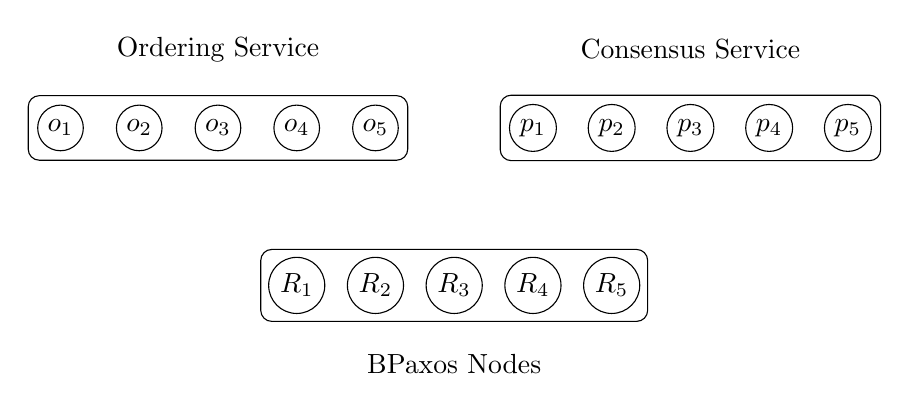
\begin{tikzpicture}
    \tikzstyle{machine}=[draw, circle, inner sep=2pt]

    % Ordering Service
    \node[machine] (o1) at (0, 2) {$o_1$};
    \node[machine] (o2) at (1, 2) {$o_2$};
    \node[machine] (o3) at (2, 2) {$o_3$};
    \node[machine] (o4) at (3, 2) {$o_4$};
    \node[machine] (o5) at (4, 2) {$o_5$};
    \node (os) at (2, 3) {Ordering Service};
    \draw[rounded corners]
      ($(o1.south west) + (-0.2, -0.2)$) rectangle
      ($(o5.north east) + (0.2, 0.2)$);

    % Consensus
    \node[machine] (p1) at (6, 2) {$p_1$};
    \node[machine] (p2) at (7, 2) {$p_2$};
    \node[machine] (p3) at (8, 2) {$p_3$};
    \node[machine] (p4) at (9, 2) {$p_4$};
    \node[machine] (p5) at (10, 2) {$p_5$};
    \node (os) at (8, 3) {Consensus Service};
    \draw[rounded corners]
      ($(p1.south west) + (-0.2, -0.2)$) rectangle
      ($(p5.north east) + (0.2, 0.2)$);

    % BPaxos Nodes
    \node[machine] (b1) at (3, 0) {$R_1$};
    \node[machine] (b2) at (4, 0) {$R_2$};
    \node[machine] (b3) at (5, 0) {$R_3$};
    \node[machine] (b4) at (6, 0) {$R_4$};
    \node[machine] (b5) at (7, 0) {$R_5$};
    \draw[rounded corners]
      ($(b1.south west) + (-0.2, -0.2)$) rectangle
      ($(b5.north east) + (0.2, 0.2)$);
    \node (bpaxos) at (5, -1) {BPaxos Nodes};
  \end{tikzpicture}

  \caption{Simple BPaxos}\figlabel{SimpleBPaxos}
\end{figure}
}

\paragraph{Instances}
As with EPaxos, every BPaxos node $R$ manages a set of numbered
\defword{instances} $R.1$, $R.2$, $R.3$, $\ldots$. As described in
\cite{moraru2013there}, we can visualize the set of instances as a
two-dimensional grid with the set of BPaxos nodes on the $x$-axis and the set
of instance numbers on the $y$-axis, as illustrated in
\figref{BPaxosInstances}.

{\begin{figure}[ht]
  \centering
  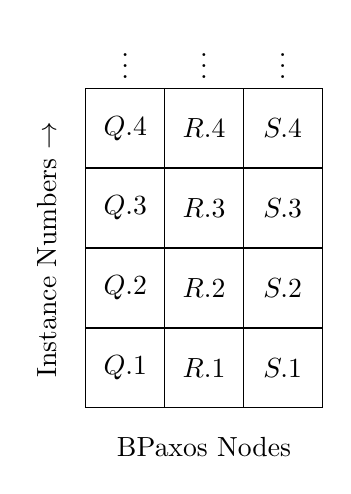
\begin{tikzpicture}
    \tikzstyle{box}=[draw, minimum width=1cm, minimum height=1cm]

    \node[box] (q1) at (0, 0) {$Q.1$};
    \node[box, above=0cm of q1] (q2) {$Q.2$};
    \node[box, above=0cm of q2] (q3) {$Q.3$};
    \node[box, above=0cm of q3] (q4) {$Q.4$};
    \node[above=0cm of q4] (qdots) {$\vdots$};

    \node[box] (r1) at (1, 0) {$R.1$};
    \node[box, above=0cm of r1] (r2) {$R.2$};
    \node[box, above=0cm of r2] (r3) {$R.3$};
    \node[box, above=0cm of r3] (r4) {$R.4$};
    \node[above=0cm of r4] (rdots) {$\vdots$};

    \node[box] (s1) at (2, 0) {$S.1$};
    \node[box, above=0cm of s1] (s2) {$S.2$};
    \node[box, above=0cm of s2] (s3) {$S.3$};
    \node[box, above=0cm of s3] (s4) {$S.4$};
    \node[above=0cm of s4] (sdots) {$\vdots$};

    \node (nodes) at (1, -1) {BPaxos Nodes};
    \node[rotate=90] (nodes) at (-1, 1.5) {Instance Numbers $\rightarrow$};
  \end{tikzpicture}
  \caption{BPaxos instances}%
  \figlabel{BPaxosInstances}
\end{figure}
}

\paragraph{Ordering Service}
\newcommand{\deps}[1]{\text{deps}(#1)}

On to the \defword{ordering service}. A BPaxos node $R$ sends a state machine
command $a$ to the ordering service for instance $R.i$. When the ordering
service receives a command $a$ for instance $R.i$, it replies with a tuple $(a,
\deps{a})$ where $a$ is the command and $\deps{a} = \set{I_1, \ldots, I_n}$ is
a set of instances that we call $a$'s \defword{dependencies}. The ordering
service provides the following guarantee. If two conflicting commands $a$ and
$b$ in instances $I_a$ and $I_b$ yield responses $(a, \deps{a})$ and $(b,
\deps{b})$ from the ordering service, then either $I_a \in \deps{b}$ or $I_b
\in \deps{a}$ (or both). That is, if two conflicting commands are sent to the
ordering service, at least one is guaranteed to be a dependency of the other.

Implementing a fault tolerant ordering service is straightforward. We employ
$2f + 1$ ordering service nodes $o_{1}, \ldots, o_{2f + 1}$. When a BPaxos node
$R$ sends a command $a$ in slot $R.i$ to the ordering service, it sends the
command to all $2f + 1$ of the ordering service nodes. Every ordering service
node $o_i$ maintains a set $O_i = {(c_1, I_1), (c_2, I_2), \ldots}$ of all the
commands and corresponding instances that it has received. When node $o_i$
receives a command $a$ for slot $I$ from a BPaxos node, it atomically performs
two actions.
%
First, $o_i$ replies to the BPaxos node with the pair $(a, \deps{a}_i)$ where
$\deps{a}_i = \setst{I}{\exists (c, I) \in O_i.\ \text{$a$ and $c$ conflict}}$
is the set of instances that $o_i$ has previously received that contain a
command that conflict with $a$.
%
Second, $o_i$ adds $a$ to $C_i$. When a BPaxos node receives replies $(a,
\deps{a}_{i_1}), \ldots, (a, \deps{a}_{i_{f+1}})$ from a quorum $Q_a$ of $f +
1$ ordering service nodes, it takes $(a, \deps{a}_{i_1} \cup \ldots \cup
\deps{a}_{i_{f+1}}) = (a, \deps{a})$ to be the response from the ordering
service.

To understand why this ordering service implementation provides its advertised
guarantees, consider conflicting commands $a$ and $b$ in instances $I_a$ and
$I_b$. Assume $a$'s reply $(a, \deps{a})$ was formed from a quorum $Q_a$ and
$b$'s reply $(b, \deps{b})$ was formed from a quorum $Q_b$. Any two quorums
intersect, so $Q_a \cap Q_b$ is nonempty. Let $o_i$ be an ordering service node
in this intersection. $o_i$ either received $a$ or $b$ first. If it received
$a$ first, then $(a, I_a)$ is in $O_i$ when $o_i$ processed command $b$, so
$o_i$ includes $I_a$ in $\deps{b}_i$, so $I_a$ is in $\deps{b}$. Symmetrically,
if $o_i$ received $b$ first, then it includes $I_b$ in $\deps{a}$.

\paragraph{Consensus Service}
Next up, the \defword{consensus service}. We assume we have some set $p_1,
\ldots, p_n$ of nodes that implement Plain Jane consensus. A BPaxos node can
propose to the consensus service that some value $v$ be chosen in some instance
$I$. The consensus service replies with the value that has been chosen in
instance $I$, which may or may not be $v$ depending on if there are concurrent
proposers proposing to instance $i$. The consensus service guarantees that for
every instance $i$, at most one value is ever chosen in $i$.

\paragraph{BPaxos Nodes}
Finally, we assume a fixed set $R_1, \ldots, R_{2f+1}$ of $2f + 1$ BPaxos
nodes.
%
Clients sends state machine commands to BPaxos nodes to be executed by the
replicated state machine. When a BPaxos node $R$ receives a command $a$, it
sends the command to the ordering service in a previously unused instance $R.i$
and receives a reply $(a, \deps{a})$. $R$ then proposes the value $(a,
\deps{a})$ to the consensus service in instance $R.i$. The consensus service
then replies with some chosen value $(a', \deps{a'})$, which is equal to $(a,
\deps{a})$ in the failure-free case. At this point, the command $a'$ is
considered committed in instance $R.i$ of the directed graph of state machine
commands with inbound edges from instances in $\deps{a'}$. Node $R$ also
informs the other BPaxos nodes that the value $(a', \deps{a'})$ has been
committed. As noted earlier, the execution of the commands in the directed
graph is identical to that of EPaxos. Committed commands are committed in
reverse topological order, one strongly connected component at a time.

\newcommand{\noop}{\text{noop}}
It's possible that (1) a committed command $a$ depends on an instance $R.i$
that contains an uncommitted command, and (2) the BPaxos node $R$ that manages
the instance $R.i$ has crashed. If the instance $R.i$ remains forever
uncommitted, then the command $a$ will never be executed. To avoid this
liveness violation, if any BPaxos node $S$ notices that instance $R.i$ has been
uncommitted for some time, it can propose to the consensus service that the
value $(\noop, \emptyset)$ be chosen in instance $R.i$ where $\noop$ is a
command that doesn't affect the state machine.

% TODO: Explain no liveness.

\paragraph{Correctness}
That's the basic version of BPaxos. We can prove it's correct by leveraging
EPaxos' proof of correctness. Open up \cite{moraru2013proof} and head to
section 5.6, which contains proofs of EPaxos' correctness.
\begin{itemize}
  \item
    \textbf{Theorem 1} says that EPaxos satisfies nontriviality. Clearly, so
    does BPaxos.

  \item
    \textbf{Lemma 1} says that EPaxos commits a command in an instance only if
    no other command will ever be committed in the same instance. The EPaxos
    proof is about two pages and not very easy to understand. However, the fact
    that BPaxos satisfies Lemma 1 is immediate from the fact that we use a
    consensus service. In fact, Lemma 1 is really just a restatement of the
    exact property that the consensus service provides.

  \item
    \textbf{Theorem 2} follows from Lemma 1.

  \item
    \textbf{Theorem 3} is trivial.

  \item
    \textbf{Theorem 4} states that if two conflicting commands are both
    committed, then they will be executed in the same order by every BPaxos
    node. The proof that BPaxos satisfies Theorem 4 is more or less the same as
    the proof that EPaxos satisfies theorem 4, which shouldn't be too
    surprising because BPaxos executes commands 100\% identically to EPaxos. In
    short, if two commands conflict, the ordering service guarantees that one
    will depend on the other. If both commands end up in the same strongly
    connected component, they will be executed in the same deterministic order.
    And, if the commands end up in different strongly connected components,
    then one component is guaranteed to be ordered before the other, so the two
    commands are executed in reverse topological order. There's also the
    wrinkle that we may commit a $\noop$, but $\noop$s don't conflict with any
    other commands, so we have nothing to worry about.
\end{itemize}

% TODO: Reference EPaxos proof and show our thing works.
% TODO: Show no liveness.

\subsection{Tweak 1: Paxos and Liveness}
% TODO: Implement consensus with Paxos. On failure, re-run paxos substituting
% no-ops if needed.
% TODO: Show liveness works now.

% \subsection{Tweak 2: Colocation}
% \subsection{Tweak 3: Enter Fast Paxos}
% \subsection{Tweak 4: Coordinated Recovery}

% \section{Comparison with EPaxos}
% TODO: quorum sizes + fast BPaxos.

\bibliographystyle{plain}
\bibliography{references}
\end{document}
